% !TeX root = ../../thesis.tex

% ~10 pages 

\chapter{Results}
\label{chap:results}

Chapter \ref{chap:design} has presented a conceptual system architecture which uses the semantic web to improve sensor data discovery as well as the integration and aggregation of sensor data from multiple sources. This has been implemented in a proof of concept implementation (Chapter \ref{chap:impl}). In the following sections the outcomes and results of this architecture are discussed (Section \ref{par:differences} to \ref{reuseOM}). Afterwards, a comparison is made with the \acf{csw} (Section \ref{compareCSW}) and with semantic sensor data middle ware (Section \ref{compareSSM}). 

\section{Implementation differences of Sensor Observation Services}
\label{par:differences}
The sources of sensor data used for the proof of concept were two \aclp{sos}. The first \ac{sos} is maintained by the \acf{rivm}. This service contains air quality sensor data for the Netherlands. The second \ac{sos} is maintained by the \ac{ircel} and contains air quality sensor data for Belgium. In the process of making an automated method for approaching these \aclp{sos} a couple of differences came to light in their implementation. Even though both use the \ac{swe} standards it turned out they are not exactly the same. 

\subsection{URI definitions}
\begin{sloppypar}
	First of all, they have different approaches for making identifiers. The \ac{rivm} has \acp{uri} for \acp{foi}, like \texttt{NL.RIVM.AQ/SPO\_F-NL00002\_00008\_101\_101}. Offerings are named like \texttt{NL.RIVM.AQ/STA-NL00002/38} and procedures like \texttt{NL.RIVM.AQ/SPP-NL\_A\_5090150901}. Their observed properties \acp{uri} are reusing the `Eionet' vocabulary by the \ac{eea} and look like: \url{http://dd.eionet.europa.eu/vocabulary/aq/pollutant/1}. The \ac{ircel} has a different approach to these identifiers. They describe \acp{foi} with \acp{uri} such as \texttt{BELAB01}. Procedures are simply assigned a five or six digit integer like \texttt{10607}. Observed properties have recieved identifiers which are a combination of letters and integers, such as \texttt{44201 - O3}. Offerings are named as a combination of observed property and procedures: \texttt{44201 - O3\_.\_6711}. Looking at both methods for creating identifiers it is clear that there is no resemblance between the two \aclp{sos}. It is not possible to automatically match the identifiers of both \aclp{sos}. This has to do with the fact that the \ac{swe} standards typically allow  any \ac{uri} to be provided, without further specification of its structure. 
\end{sloppypar}

\subsection{Content of response document}
\begin{sloppypar}
Another difference between the two \aclp{sos} is that they supply different kinds of content in their response documents. For example, offering definitions in the capabilities document from \ac{ircel} contain bounding boxes to provide an indication of their geographical coverage. However, the capabilities document by the \ac{rivm} does not provide any data related to the physical locations at all. The \texttt{DescribeSensor} responses by the \ac{ircel} include a point geometry as part of the sensor's metadata, while the \ac{rivm} provides the \ac{foi} identifier for which the geometry can be retrieved using a a \texttt{GetFeatureOfInterest} request. This \texttt{GetFeatureOfInterest} request by \ac{ircel} returns the geometries of \acp{foi} with \acp{crs} in the \texttt{urn:ogc:def:nil:OGC:unknown} format. The \ac{sos} by the \ac{rivm} returns geometries of \acp{foi} with \acp{crs} in the \texttt{http://www.opengis.net/def/nil/OGC/0/unknown} format. 
\end{sloppypar}

\begin{sloppypar}
Another implementation difference is visible in the \texttt{GetObservation} response documents. When retrieving sensor data from the \ac{sos} using \texttt{GetObservation} requests \ac{ircel} provides this data as an array of comma separated values, using the \ac{swe} Array Observation class. With this method all metadata that is shared by observations from the same sensor (observed property, procedure, \ac{foi}, \ac{uom}) are only defined once in the response document. The \ac{rivm} on the other hand, provides the observation data embedded in \ac{xml} tags using the \ac{om} Measurement class. With this approach all observations are self describing, defining the metadata of a sensor for each observation it makes.   
\end{sloppypar}

\begin{sloppypar}
	All these differences have caused the proof of concept described in Chapter \ref{chap:impl} to become more complex than initially expected. Providing a \texttt{describeSensor} document with as much information as possible (containing related features of interest, observed property and offerings) is especially important for making sense of the metadata. Working with response documents is much easier if the appropriate \ac{sensorml} classes are being used to describe sensor metadata, instead of adding it to the more general \texttt{swe:keywords}, or abstract section for example. It is not inconsistent with \ac{swe} standards to include metadata in one of these ways, but it does not create machine understandable content. 
\end{sloppypar}


\section{Semantics in Sensor Observation Services}
The metadata in \aclp{sos} do not necessarily contain semantic \acp{uri} as identifiers. Therefore the workflow of Chapter \ref{chap:design} includes a process for creating these semantic \acp{uri} based on the \ac{swe} \ac{xml} schemas. However, two issues occurred. First of all, identifiers are used in a \ac{sos} which are completely meaningless, especially from a machine readable point of view. The lack of well defined observable properties and procedures are the main problem, as they combined with a \ac{foi} represent a deployed sensor. Secondly, there is a lot of complexity involved in automatically creating \acp{uri} for metadata, where each \ac{uri} is unique, compact and valid. These two issues will be further discussed in the following subsections. 

\subsection{Mapping of observable properties}
In Section \ref{par:differences} the differences between identifiers in the \aclp{sos} by \ac{ircel} and the \ac{rivm} have been described. They are compliant with the \ac{swe} standards, which require any \ac{uri} regardless of semantics. The workflow of Chapter \ref{chap:design} uses the sensor location, temporal range and observed property as the main elements of the logical query input. Therefore, ill-defined procedures and observed properties are problematic when automatically retrieving (meta)data from different services. Both \aclp{sos} used in this thesis had non-machine understandable identifiers. The vocabulary used by the \ac{rivm} for observed properties is a step in the right direction, as it provides a textual description. However, these identifiers do not resolve to an \ac{rdf} document, but to the \ac{eea} website. This is therefore a human understandable solution. The \ac{sos} by \ac{ircel} contains identifiers which are a string of seemingly random characters, ending with an abbreviation of the observable property involved. This is partly human understandable.   

Identifying which observable properties in one \ac{sos} are the same as observable properties found in another \ac{sos} was not automatically possible in this case. It could be achieved with a minimum of semantics, such as an \ac{rdf} document containing just a triple. For example, the \texttt{owl:sameAs} predicate can be used to link to a semantic ontology, or the \texttt{foaf:name} predicate can be used to store at least the full name of the observable property. As such, by assigning just a single triple to a \ac{uri} it also already possible for an automatic process to find out which \acp{uri} represent the same observable property. 

 A manual mapping had to be implemented, because the implementation was currently not able to automatically create linked data from the metadata of a \ac{sos} using just the \ac{http} address as input. This manual mapping is a small \ac{rdf} document containing one triple for every observable property \ac{uri}, using the \texttt{owl:sameAs} predicate to link it to the corresponding DBPedia definition. The proof of concept implementation takes both the \ac{http} address of the \ac{sos} and this manual mapping as input.          

\subsection{Automatically creating URIs}
The method presented in this thesis includes a process to automatically assign \acp{uri} to non-semantic data and to define \acp{uri} for concepts that are implicitly stored in a \ac{sos}. For example, a \ac{sos} could contain one procedure and ten \acp{foi}. The deployed sensors are implicitly represented by combining the procedure with a \ac{foi}, although they are not part of the \ac{sos} \ac{xml} schemas. If an \ac{uri} is automatically created for data from an unknown source, there is an amount of uncertainty about what the resulting \acp{uri} will look like. A random identifier can be used, or the identifier that is already provided by the data source. This identifier will most likely contain some reference to the nature of the real world object the \ac{uri} represents. Therefore, this could be preferred to a completely random identifier. However, as shown in Section \ref{par:differences} identifiers can also be random or non-semantic \acp{url}. Since the \ac{om} schema allows simply any \ac{uri}, very long and strange \acp{uri} can be created when adding the given identifier to the \ac{uri}. 

Therefore, the proof of concept implementation used a combination of random and existing identifiers. It uses the name of the \ac{sos} organisation (`RIVM', `Ircel-Celine'), the type of metadata (`procedure', `FOI') and a random integer ranging from zero to the amount of instances of this type. However, this is not a watertight solution either, because the name of the organisation could create an invalid \ac{url}. In the proof of concept invalid characters and spaces had to be escaped to prevent this. The name of the organisation was selected over the title of the \ac{sos}, since those are often very verbose. Nevertheless, using the name of the organisation the problem could arise that multiple \aclp{sos} are maintained by the same organisation. This could lead to non-unique identifiers. 

\section{Missing classes in linked data ontologies}

A sensor has a large amount of metadata, which can be retrieved from a \ac{sos}. First of all, there is metadata according to the \ac{swe} schemas. This defines aspects, such as observed property, \ac{foi} and procedure, which can be described using om-lite and sam-lite ontologies (see Subsection \ref{omsamlite}, Appendix \ref{map:getFOI} and Appendix \ref{map:capabilities}). Secondly, the \ac{sos} instance and its functionality are also part of a sensors metadata. However, a number of these metadata classes are missing in the linked data ontologies. There is for example, not a description of what a \ac{sos} is, which request and response formats they support, and what offerings are.

To overcome this issue in the proof of concept, the PROV ontology has been used to describe these classes on a more abstract level. As shown in Section \ref{prov-o}  \aclp{sos}, sensors, \acp{foi} and procedures can be described in terms of \texttt{Entities}, \texttt{Agents} and \texttt{Activities}. Appendix \ref{map:SOS} provides an overview of how these instances are mapped to the PROV ontology. To link output formats and sensors to a \ac{sos}, some basic Dublin Core\footnote{\url{http://purl.org/dc/terms/}} classes have been used as well, such as \textit{hasFormat} and \textit{isPartOf}. These ontological classes have helped providing a minimal definition. It enabled a \ac{sparql} query to retrieve the required information from the endpoint. However, the proof of concept knows that it only contained \ac{sos} metadata. The metadata itself is not sufficiently defined. If a web process does not know in advance that \ac{sos} metadata is described by the semantic knowledge base, it would not be able to find this out on its own. 

\section{Spatial queries with SPARQL}
\label{par:spQueries}
Spatial queries are an essential part of the method presented in this thesis. They are used in the process of selecting which sensors are spatially relevant to the user's data request. However, the proof of concept implementation showed that the performance of vector geometries in \ac{sparql} is not optimal. Also, the order of latitude and longitude in point coordinates turned out to be a problem. In the next two subsections these issues will be discussed, together with the implemented solutions.     

\subsection{Vector queries with SPARQL}
The workflow described in Section \ref{par:logicalDesign} starts with discovering metadata of sensors which are inside a spatial feature. This feature can be a raster cell or vector geometry. Spatial \ac{sparql} queries with raster cells are relatively fast. However, with vector geometries the performance is lacking when large amounts of data are being retrieved. The endpoint has limited its ability to receive queries to a maximum amount of characters per query. Vector geometries can easily exceed this length. Therefore, three methods for spatial querying have been implemented to retrieve metadata of sensors inside a vector feature. First of all, a method has been implemented which creates \ac{sparql} queries with a spatial filter expression containing the original vector geometries. Secondly, an alternative has been implemented which creates \ac{sparql} queries in which \ac{eea} raster cells overlapping the vector geometry are added to a spatial filter expression. Thirdly, an approach is tested in which the spatial querying is performed on the \ac{sos} side using spatial filters in \texttt{GetObservation} requests. The three methods are described in more detail below.

The \ac{wps} does not have to perform any further spatial queries with the first method. A single query retrieves the metadata of sensors inside the geometry. This is a fast procedure, since it uses a Postgres database in combination with the Postgis extension. Responding to a \ac{sparql} query with a spatial filter is a matter of seconds in the proof of concept implementation. However, when more complicated vector geometries are used, the \ac{wkt} definition gets more verbose. This can lead to a rejection of the query by the endpoint, as it exceeds a maximum amount of characters defined by the server. The method has been tested with Strabon and Parliament endpoints, since both of them handle spatial \ac{sparql} queries. The Strabon endpoint has been used in the final proof of concept, because it handled long queries better. However, queries still get rejected if complicated vector geometries are added to the filter expression.    

The second method performs a rough spatial filtering at the side of the endpoint and the detailed spatial filtering at the \ac{wps} side. To do this, raster cells overlapping the vector geometries are added to the \ac{sparql} filter. The returned sensor metadata is then filtered by the \ac{wps} using the Shapely Python package. The advantage of this method is that it always works, regardless of the geometries which are used as input. However, the downside is that it introduces an extra step in the process of retrieving metadata. This results in a lower performance of the entire process of retrieving sensor metadata.  

The third method retrieves addresses of \aclp{sos} that have metadata in a certain area from the endpoint. To these returned addresses a \texttt{GetObservation} request is sent with a spatial filter. The problem encountered with this method is the difference in filtering capabilities between \aclp{sos}. Not all services had spatial filters implemented. If these filters would have been implemented by all \aclp{sos} it could have been a viable alternative. However, another disadvantage of this method is that only a very rough spatial filtering is applied on the endpoint side using a bounding box, since the detailed spatial filtering happens on the \ac{sos} side. Therefore, \aclp{sos} might have sensors inside the bounding box of the vector geometry, but not inside the vector geometry itself. This leads to unnecessary requests to those services \aclp{sos}, lowering the performance of the entire process of retrieving sensor data.

Considering all advantages and disadvantages of the three methods the proof of concept implementation selects the second method by default. The other methods can be selected using an optional input parameter. 

\subsection{Latitude and longitude order in point coordinates}
The proof of concept implementation had to be adjusted to cope with inconsistencies regarding the order in which latitude and longitude are being presented. The \ac{sos} of the \ac{rivm} provides point geometries as longitude, latitude. However, the Strabon endpoint expects the order to be latitude, longitude. The coordinates by \ac{ircel} do use the latitude, longitude order. Mixing up the order of a point coordinate results in wrong outcomes of spatial queries. The biggest issue with the coordinate order is that there is no description of it in the \ac{crs} specification.  The order of longitude and latitude should be decided upon by the geomatics and geospatial community or explicitly defined to prevent confusion. 

However, to make the current proof of concept work an ad hoc solution has been implemented based on a remark by \cite{GEO:GDAL}: coordinates defining their \ac{crs} in the format of \texttt{urn:ogc:def:crs:EPSG:unknown} are generally using the longitude, latitude order. Coordinates defining their \ac{crs} in the format of \texttt{http://www.opengis.net/def/nil/OGC/0/unknown} are generally using the latitude, longitude order. Therefore, the order is swapped for geometries with the former \ac{crs} format. The coordinates which use the latter format for their \ac{crs} are left as they are. \cite{GEO:TOOLS} describes that in theory the format of a \ac{crs} \ac{uri} has nothing to do with the latitude and longitude order. Therefore, there is no guarantee that this solution will continue to work over time as it is not part of any specification. Still, this approach works for the \aclp{sos} used in this thesis, but it is not the preferred solution.   

\section{Reusing the OM Observation Schema for output data}
\label{reuseOM}
After sensor data is retrieved from the \aclp{sos} and further processed, it is returned to the user as a \ac{json} or \ac{xml} file. The content of these documents are structured according to the \ac{om} schema. However, this schema cannot be (re)used when data from different procedures has been used to create a single aggregated value. The \aclp{sos} by the \ac{rivm} and \ac{ircel} both use different procedures for their observations. A procedure is defined in \ac{om} as a method, algorithm or instrument, or a system of these. A procedure can therefore be a sensor, an algorithm processing the raw observation data and/or a system of sensors observing a property of the \ac{foi}. It could be discussed to what extent it is problematic for different procedures which observe the same property of a \ac{foi} to be aggregated into a single value. The answer to this question could differ from one procedure to the other and should be answered by people with expert knowledge on the exact functioning of sensing procedures. It could also be semantically stored as suggested by \cite{SSW:Stasch4} to allow this knowledge to be machine understandable. The method designed in this thesis can then be extended to make these decisions based on semantics about sensing procedures. 

In the current proof of concept implementation all sensors observing the same property of their \acp{foi} can be aggregated together. This decision makes it possible to integrate and aggregate sensor data, retrieved from multiple sources, before it is returned to the user. However, the problem remains that the procedure element of the \ac{om} observation schema cannot be added with different procedures. According to the \ac{xml} specification, the procedure is nillable, but only \enquote{where the information, though strictly required, is not available} \citep[p. 42]{SW:OGC8}. This is not the case for the observations used in this thesis, they provide \acp{uri} for their procedures. In the proof of concept the procedure element is left out of the response documents, but this is not in line with the \ac{om} schema. Therefore, the schema should allow the procedure element to contain multiple observation procedures or another kind of value to describe the origin of the observation data. 

As a workaround for dealing with procedures of aggregated data, the aggregation could be seen as part of a larger observation system, starting at the sensors, and via the \ac{sos} going into an (aggregation) algorithm to produce the observation result. This system would then be given a unique \ac{uri} which is placed in the response document. This `system' would be imagined ad hoc, only when a user's query is received. When only a \ac{urn} is returned -- which suffices for the \ac{om} observation schema -- this is a relatively simple workaround, but the semantics which might have been present, are then lost. When semantics are required for procedure definitions, \ac{rdf} documents containing descriptions of the origin of the data should be created on-the-fly for every request. Whether this is a desirable and viable solution for including aggregated data in the \ac{om} observation schema should be further researched.        

\section{Comparison with a Catalog Service for the Web}
\label{compareCSW}
In Subsection \ref{par:CSW} the \acl{csw} has been described. This is a web service standard for discovering other geo web services, such as \ac{wfs} and \ac{wcs}. For including \aclp{sos} in these catalogs \cite{SW:OGC4} and \cite{SW:OGC3} have developed the \ac{sir} and \ac{sor} extensions. When the method of this thesis is compared with \ac{sir} and \ac{sor}, a lot of similar functionalities can be observed. First of all, there are harvesting functions present, requiring an \ac{http} address of a \ac{sos} as input to retrieve sensor metadata. Also, the metadata is stored in a central location, providing users with an overview of available data and services. Furthermore, requests can be made for retrieving metadata about a subset of the sensors, which share certain properties. These are all characteristics of the \ac{csw} in combination with \ac{sir} and \ac{sor}, as well as of the conceptual system architecture described in Chapter \ref{chap:design}.  

However, there are also some considerable differences between the \ac{csw} and a semantic knowledge base. For example, the \ac{csw} does not necessarily support the same level of semantics which is required in a semantic knowledge base. The \ac{sir} harvesting procedure retrieves metadata from \aclp{sos} according to the \ac{swe} \ac{xml} schemas and this data is just transferred to another web service. The method presented in this thesis maps these \ac{xml} schemas for \ac{sos} metadata to linked data ontologies. This adds meaning and allows it to be machine understandable.

A second difference is the platform used for retrieving sensor metadata. The \ac{csw} is an \ac{ogc} web service, from which data can be retrieved by sending \ac{csw} requests, such as \texttt{GetCapabilities}, \texttt{DescribeRecord} or \texttt{GetRecord}. The client should know the exact \ac{http} address of the \ac{csw} as well as how to communicate with it. The method in this thesis creates linked data which is stored in a endpoint on the semantic web. Data from an endpoint can be queried using the \ac{sparql} query language. It can also be linked to and from other related data, which allows it to be discovered more easily.    

The data model behind the \ac{swe} and \ac{csw} services are based on the closed world assumption. This means that the application is supposed to have complete information at its disposal with respect to the observation data. However, the semantic web is based on the open world assumption. In this case, currently unknown or unavailable information is not viewed as non-existing. The semantic knowledge base allows other data which is directly or indirectly related to (the context of) an observation to be part of the data model. This allows semantic reasoning based on a combination of \ac{swe} related data and non-\ac{swe} related data.       

In their current implementation the \ac{sir} and \ac{sor} allow any \ac{swe} web service to be included in a \ac{csw}. Also \aclp{sps}, \aclp{sas} and \aclp{wns} can be looked up using a \ac{csw}. These standards have not been taken into consideration for this thesis. Because of time limitations the method presented here focusses only on the \ac{sos}. However, the principles described here can be used to extend it to include any other \ac{swe} web services in the future as well (see Chapter \ref{chap:futureResearch}).        

\section{Comparison with semantic sensor middleware}
\label{compareSSM}
The method presented in this thesis could also be compared to the so-called semantic sensor middleware as described in Section \ref{par:middleware}. These middlewares create a layer on top of a \ac{sos}, allowing them to output their contents semantically enriched. Examples of this are the \acf{semsos} service by \cite{SSW:Henson} and \cite{SSW:Pschorr}, and the \acf{sel} by \cite{SSW:Janowicz}. These middlewares offer similar functionality to the method presented in this thesis as they add semantics to sensor metadata. In the backend they use a linked data model that allows the \ac{sos} to return semantic data based on the \ac{om} data model. 

\begin{figure}
	\centering
	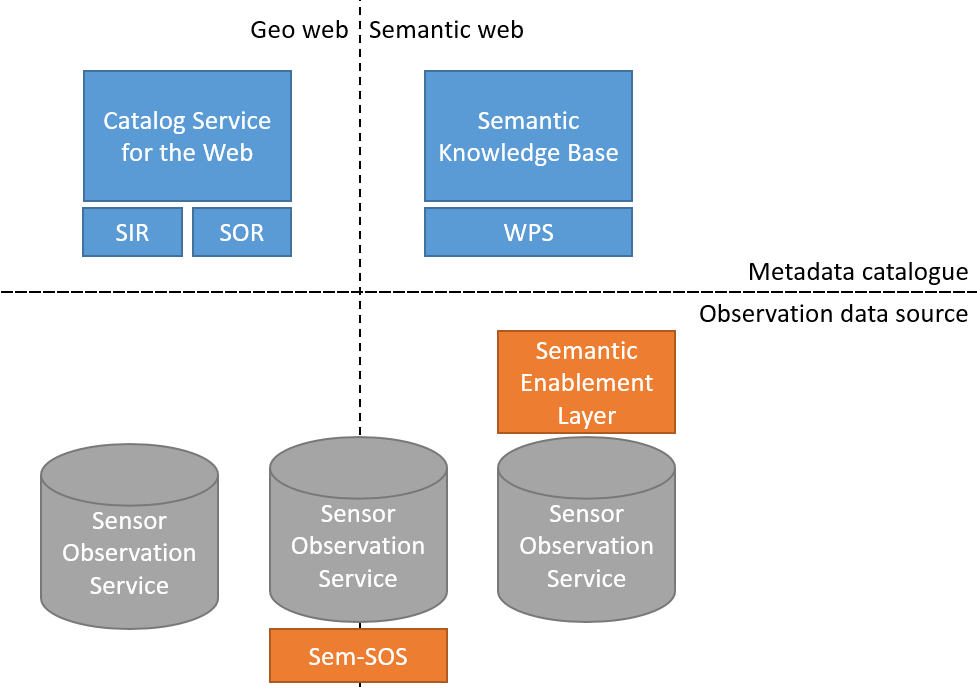
\includegraphics[width=0.8\linewidth]{figs/catalogVSsource.PNG}
	\caption{Distinction between solutions for metadata catalogues and observation data sources}
	\label{fig:catVSsource}
\end{figure}

A key difference between the semantic sensor middleware approaches and the method presented in this thesis is that the \ac{semsos} and \ac{sel} are enriching a single \ac{sos} with semantics. This thesis has a different scope, where metadata of multiple \aclp{sos} are combined, providing an overview which allows for discovering and understanding sensor data (Figure \ref{fig:catVSsource}). The \ac{wps} performs the tasks of discovering, retrieving, integrating and aggregating data, lowering the burden on users. A semantic sensor middleware has not been created to automatically discover and retrieve observation data, but focuses on making the \ac{sos} data accessible with added semantics or in the \ac{rdf} format. In the case of \ac{semsos} and \ac{sel} one or more request will still have to be made to a \ac{sos} to decide whether the service is relevant to a user's logical data request, unless it is connected to a \ac{csw}. By explicitly storing the metadata in a semantic knowledge base instead of a semantically enriched \ac{sos} service, this question can be answered with \ac{sparql} queries to the endpoint. Furthermore, the method described in this thesis does not only describe data semantically, but also makes it discoverable by adding links from another semantic knowledge base (DBPedia). This increases the chances for observation metadata to be discovered.        

The advantage of the middleware approaches is that data is not duplicated, but only returned in a different format. Duplicated data can become out of sync with their source, creating a situation where multiple versions of the same data are available online. To prevent this issue the data has to be frequently updated. Alternatively, it could also be retrieved directly from the source instead of duplicating it. The \ac{semsos} and \ac{sel} provide a method for retrieving \ac{rdf} data about observations directly from the \ac{sos} source.


\section{Concluding remarks}
In Chapter \ref{chap:design} a conceptual system architecture has been presented. This architecture has been tested using a proof of concept implementation, combining geo web and semantic web standards. The results of this proof of concept show that the conceptual system architecture can be implemented, creating a semantic knowledge base with sensor metadata combined from different \aclp{sos}. However, a number of issues have also surfaced with respect to the \ac{swe} standards. There are differences in the use of \ac{swe} standards between \aclp{sos} and there is not always a sufficient description of the metadata. This makes it difficult for other users (both human users and automated processes) to understand the metadata. Another issue is the complexity which is involved in creating completely automated processes for outputting linked data of \ac{sos} metadata. The data is retrieved from multiple sources and there can be differences in the way these sources have structured it. 

The functionality of a semantic knowledge base has also been compared with the \ac{csw} and (through middleware) semantically enriched \aclp{sos}. As Figure \ref{fig:catVSsource} shows, the \ac{csw} and a semantic knowledge base are both in the domain of metadata cataloguing. They harvest metadata from sources to provide a broad overview of all available data. Semantic sensor middleware layers can be used to add semantics to an individual data source. The use of semantic sensor middleware and a semantic knowledge base are therefore not mutually exclusive. 

%Performance optimisation has been beyond the scope of this thesis: The presented conceptual system architecture focused solely on the functionality. However, the proof of concept does provide an indication of the order of magnitude and potential performance bottlenecks. Currently, the retrieval of metadata using \ac{sparql} queries is a matter of seconds, using a Strabon endpoint, metadata from two \aclp{sos}, and the queries described in Subsection \ref{par:discoverSensors}. The retrieval of observation data can go up to a number of minutes, depending largely on the amount of sensors and sources, and the requested temporal range. 

   
